\documentclass[tikz]{standalone}
\usepackage{tikz}
\usetikzlibrary{patterns,snakes,angles}
 
\begin{document}
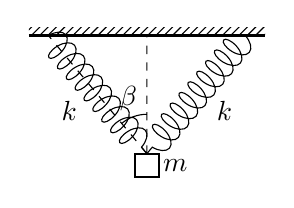
\begin{tikzpicture}
	\draw [draw=none, pattern=north east lines] (0,0) rectangle (3,0.1);
	\draw [thick] (0,0) -- (3,0);
	\draw [snake=coil, segment amplitude=5pt, segment length=5pt] (0.25,0) -- (1.5, -1.5) node [midway, below=6pt, left = 4pt] {$k$};
	\draw [snake=coil, segment amplitude=5pt, segment length=5pt] (2.75,0) -- (1.5, -1.5) node [midway, below=6pt, right =4pt] {$k$};
	\draw [thick] (1.35, -1.5) rectangle (1.65,-1.8) node [right=6pt, above=-1.5pt] {$m$};
	\coordinate (A) at (1.5,0);
	\coordinate (B) at (1.5,-1.5);
	\coordinate (C) at (0.25,0);
	\draw [dashed] (B)--(A) (B)--(C);
	\pic [draw, -, angle eccentricity=5] {angle = A--B--C};
	\node [above=20pt, left = 0pt] at (B) {$\beta$};

\end{tikzpicture}
\end{document}